\documentclass[oneside,graybox,envcountchap,sectrefs]{svmono}


\usepackage{mathptmx}
\usepackage{helvet}
\usepackage{courier}
\usepackage{braket} % used for Dirac notation
\usepackage{algorithmicx}
\usepackage{algpseudocode} % together for code
\usepackage{amsfonts}
\usepackage{amsmath}
\usepackage{simplewick}
\usepackage{type1cm}         
\usepackage{exercise}
\usepackage{makeidx}         % allows index generation
\usepackage{graphicx}        % standard LaTeX graphics tool
                             % when including figure files
\usepackage{multicol}        % used for the two-column index
\usepackage[bottom]{footmisc}% places footnotes at page bottom
\usepackage[usenames,dvipsnames,x11names]{xcolor}
 \usepackage{listings}
 \usepackage{epic}
 \usepackage{eepic}
 \usepackage{a4wide}
 \usepackage{color}
 \usepackage{amsmath}
 \usepackage{amssymb}
 \usepackage[T1]{fontenc}
 \usepackage{cite} % [2,3,4] --> [2--4]
 \usepackage{shadow}
 \usepackage{hyperref}
 \usepackage{bezier}
 \usepackage{pstricks}
%\usepackage{refcheck}
\setcounter{tocdepth}{2}
\usepackage{textcomp,type1ec,pdfpages}
\usepackage{bera}
\usepackage{slashed}
\usepackage{environ}
\usepackage{esvect}
\usepackage{xspace}
\usepackage{bm}


%\usepackage{natbib}
\usepackage{chapterbib}
\definecolor{dkgreen}{rgb}{0,0.6,0}
\definecolor{gray}{rgb}{0.5,0.5,0.5}
\definecolor{mauve}{rgb}{0.58,0,0.82}

 \lstset{language=c++}
 \lstset{alsolanguage=[90]Fortran}
 \lstset{alsolanguage=python}
% \lstset{basicstyle=\small}
 \lstset{backgroundcolor=\color{white}}
 \lstset{frame=single}
 \lstset{stringstyle=\ttfamily}
 \lstset{keywordstyle=\color{red}\bfseries}
 \lstset{commentstyle=\itshape\color{blue}}
 \lstset{showspaces=false}
 \lstset{showstringspaces=false}
 \lstset{showtabs=false}
 \lstset{breaklines}
 

% Default settings for code listings
% \lstnewenvironment{Python}[1]{
\lstset{%frame=tb,
  language=c++,
  alsolanguage=python,
  %aboveskip=3mm,
 % belowskip=3mm,
  showstringspaces=false,
  columns=flexible,
  basicstyle={\footnotesize\ttfamily},
  numbers=none,
  numberstyle=\tiny\color{gray},
  commentstyle=\color{dkgreen},
  stringstyle=\color{mauve},
 frame=single,  
  breaklines=true,
  %%%% FOR PYTHON 
  otherkeywords={\ , \}, \{},
  keywordstyle=\color{blue},
  emph={void, ||, &&, break, class,continue, delete, else,
  for, if, include, return,try,while},
  emphstyle=\color{black}\bfseries,
  emph={[2]True, False, None, self},
  emphstyle=[2]\color{dkgreen},
  emphstyle=[2]\color{red},
  emph={[3]from, import, as},
  emphstyle=[3]\color{blue},
  upquote=true,
  morecomment=[s]{"""}{"""},
  commentstyle=\color{green}\slshape, %%% cambie gray por green
  emph={[4]1, 2, 3, 4, 5, 6, 7, 8, 9, 0},
  emphstyle=[4]\color{blue},
  breakatwhitespace=true,
  tabsize=2
}

\renewcommand{\lstlistlistingname}{Code Listings}
\renewcommand{\lstlistingname}{Code Listing}
\definecolor{gray}{gray}{0.5}
\definecolor{green}{rgb}{0,0.5,0}

\lstnewenvironment{Python}[1]{
\lstset{
language=python,
basicstyle=\footnotesize\setstretch{1},
stringstyle=\color{red},
showstringspaces=false,
alsoletter={1234567890},
otherkeywords={\ , \}, \{},
keywordstyle=\color{blue},
emph={access,and,break,class,continue,def,del,elif ,else,%
except,exec,finally,for,from,global,if,import,in,is,%
lambda,not,or,pass,print,raise,return,try,while},
emphstyle=\color{black}\bfseries,
emph={[2]True, False, None, self},
emphstyle=[2]\color{red},
emph={[3]from, import, as},
emphstyle=[3]\color{blue},
upquote=true,
morecomment=[s]{"""}{"""},
commentstyle=\color{dkgreen}\slshape, % el color era gray pero lo cambie a verde
emph={[4]1, 2, 3, 4, 5, 6, 7, 8, 9, 0},
emphstyle=[4]\color{blue},
framexleftmargin=1mm, framextopmargin=1mm, rulesepcolor=\color{blue},
breakatwhitespace=true,
tabsize=2
}}{}


\lstnewenvironment{C++}[1]{
\lstset{
language=c++,
% basicstyle=\ttfamily\small\setstretch{1},
basicstyle=\footnotesize\setstretch{1},
stringstyle=\color{red},
showstringspaces=false,
alsoletter={1234567890},
otherkeywords={\ , \}, \{},
keywordstyle=\color{blue},
emph={access,and,break,class,continue,def,del,elif ,else,%
except,exec,finally,for,from,global,if,import,in,is,%
lambda,not,or,pass,print,raise,return,try,while},
emphstyle=\color{black}\bfseries,
emph={[2]True, False, None, self},
emphstyle=[2]\color{red},
emph={[3]from, import, as},
emphstyle=[3]\color{blue},
upquote=true,
morecomment=[s]{"""}{"""},
commentstyle=\color{dkgreen}\slshape, % el color era gray pero lo cambie a verde
emph={[4]1, 2, 3, 4, 5, 6, 7, 8, 9, 0},
emphstyle=[4]\color{blue},
% literate=*{:}{{\textcolor{blue}:}}{1}%
% {=}{{\textcolor{blue}=}}{1}%
% {-}{{\textcolor{blue}-}}{1}%
% {+}{{\textcolor{blue}+}}{1}%
% {*}{{\textcolor{blue}*}}{1}%
% {!}{{\textcolor{blue}!}}{1}%
% {(}{{\textcolor{blue}(}}{1}%
% {)}{{\textcolor{blue})}}{1}%
% {[}{{\textcolor{blue}[}}{1}%
% {]}{{\textcolor{blue}]}}{1}%
% {<}{{\textcolor{blue}<}}{1}%
% {>}{{\textcolor{blue}>}}{1},%
framexleftmargin=1mm, framextopmargin=1mm, rulesepcolor=\color{blue},
breakatwhitespace=true,
tabsize=2
}}{}
\usepackage{calrsfs}
\DeclareMathAlphabet{\pazocal}{OMS}{zplm}{m}{n}
\newcommand {\bea}{\begin{eqnarray}}
\newcommand {\eea}{\end{eqnarray}}
\newcommand {\be}{\begin{equation}}
\newcommand {\ee}{\end{equation}}
\newcommand{\beq}{\begin{eqnarray}}
\newcommand{\eeq}{\end{eqnarray}}
\newcommand {\bc}{\begin{center}}
\newcommand {\ec}{\end{center}}
\def\lsim{\mathrel{\rlap{\lower4pt\hbox{\hskip1pt$\sim$}}
    \raise1pt\hbox{$<$}}}               
\def\gsim{\mathrel{\rlap{\lower4pt\hbox{\hskip1pt$\sim$}}
    \raise1pt\hbox{$>$}}}  


\makeindex             % used for the subject index
                       % please use the style svind.ist with
                       % your makeindex program

%%%%%%%%%%%%%%%%%%%%%%%%%%%%%%%%%%%%%%%%%%%%%%%%%%%%%%%%%%%%%%%%%%%%%

\begin{document}
\frontmatter

\begin{titlepage}
\title{Introducing Computing in your Science Curriculum}
 \subtitle{A practical guide}
\date{Spring 2018}
\author{Marcos Daniel Caballero and Morten Hjorth-Jensen}
\end{titlepage}

\maketitle
\preface
Using this book, we aim to provide a practical guide for those looking to integrate computation into their undergraduate physics courses. The book will attempt to achieve several goals:
\begin{enumerate}
\item Provide motivation and rationale for why such computational integration is necessary, and as such, offer arguments in favor of computational integration that others may use for their own discussions.
\item Offer a suite of computational learning goals at a variety of scales and for a variety of topics in order to present the variety of ways and different levels of the depth t\item  which students may work with computational ideas.
\item Provide example activities in which students are engaged with such learning goals to varying degrees in order to demonstrate the wide variety of ways in which computation can be used in classrooms.
\item  Through these examples, discuss a variety of implementation models in order to inform readers of the needs, benefits, and challenges of each.
\item Discuss more broadly the issues of computational integration including available resources and on-going research efforts.
\end{enumerate}
\tableofcontents
\mainmatter
\chapter{What do we mean by computing}
\section*{Introduction: Scientific and educational motivation}

Numerical simulations of various systems in science are central to our
basic understanding of nature and technology.
The increase in computational power,
improved algorithms for solving problems in science, as well as access
to high-performance facilities, allow researchers to study
complicated systems across many length and energy scales. Applications
span from studying quantum physical systems in nanotechnology and the
characteristics of new materials or subatomic physics at its smallest
length scale, to simulating galaxies and the evolution of the universe.
In between, simulations are key to understanding
cancer treatment and how the brain works,
predicting climate changes and this week's weather,
simulating natural disasters, semi-conductor devices,
quantum computers, as well as assessing risk in the insurance and
financial industry.


\paragraph{Computing competence.}
Computing means solving scientific problems using computers. It covers
numerical as well as symbolic computing. Computing is also about
developing an understanding of the scientific process by enhancing
algorithmic thinking when solving problems.  Computing competence has
always been a central part of education in the sciences and engineering disciplines.

On the part of students, this competence involves being able to:

\begin{itemize}
\item understand how algorithms are used to solve mathematical problems,

\item derive, verify and implement algorithms,

\item understand what can go wrong with algorithms,

\item use these algorithms to construct reproducible scientific outcomes and to engage in science in ethical ways, and

\item think algorithmically for the purposes of gaining deeper insights about scientific problems.
\end{itemize}

\noindent
All these elements are central for maturing and gaining a better understanding of the scientific process.

The power of the scientific method lies in identifying a given problem
as a special case of an abstract class of problems, identifying
general solution methods for this class of problems, and applying a
general method to the specific problem (applying means, in the case of
computing, calculations by pen and paper, symbolic computing, or
numerical computing by ready-made and/or self-written software). This
generic view on problems and methods is particularly important for
understanding how to apply available, generic software to solve a
particular problem.

Computing competence represents a central element
in scientific problem solving, from basic education and research to
essentially almost all advanced problems in modern
societies. Computing competence is central to further
progress. It enlarges the body of tools available to students and
scientists beyond classical tools and allows for a more generic
handling of problems. Focusing on algorithmic aspects results in
deeper insights about scientific problems.





\paragraph{Why should basic university education undergo a shift towards modern computing?}
\begin{itemize}
\item Algorithms involving pen and paper are traditionally aimed at what we often refer to as continuous models.

\item Application of computers calls for approximate discrete models.

\item Much of the development of methods for continuous models are now being replaced by methods  for discrete models in science and industry, simply because much larger classes of problems can be addressed with discrete models, often also by simpler and more generic methodologies.
\end{itemize}

\noindent
However, verification of algorithms and understanding their limitations requires much of the classical knowledge about continuous models.

So, why should basic university education undergo a shift towards modern computing?

The impact of the computer on mathematics and science is tremendous: science and industry now rely on solving mathematical problems through computing.
\begin{itemize}
\item Computing can increase the relevance in education by solving more realistic problems earlier.

\item Computing through programming can be excellent training of creativity.

\item Computing can enhance the understanding of abstractions and generalization.

\item Computing can decrease the need for special tricks and tedious algebra, and shifts the focus to problem definition, visualization, and "what if" discussions.
\end{itemize}

\noindent
The result is a deeper understanding of mathematical modeling and the scientific method (we hope, and here our physics education research group can play a central role in promoting this).
Not only is computing via programming a very powerful tool, it can also be a great pedagogical aid.

For the mathematical training, there is one major new component among the arguments above: understanding abstractions and generalization. While many of the classical methods developed for continuous models are specialized for a particular problem or a narrow class of problems, computing-based algorithms are often developed for problems in a generic form and hence applicable to a large problem class.


Computing competence represents a central element in scientific problem solving, from basic education and research to essentially almost all advanced problems in modern societies. It enlarges the body of tools available to students and scientists beyond classical tools and allows for a more generic handling of problems. Focusing on algorithmic aspects results in deeper insights about scientific problems.

Moreover, today's projects in science and industry tend to involve larger teams. Tools for reliable collaboration must therefore be mastered (e.g., version control systems, automated computer experiments for reproducibility, software and method documentation).



\chapter{Developing learning outcomes and assessment programs} 



\section*{General learning outcomes for computing competence}

Below, we articulate high-level learning outcomes that we expect students to develop through comprehensive and coordinated instruction in numerical methods over the course of their bachelor's program at Michigan State. These learning outcomes are different from specific learning goals in that the former reference the end state that we aim for students to achieve. The latter references the specific knowledge, tools, and practices with which students should engage and discusses how we expect them to participate in that work. We reserve the discussion of specific learning goals to individual course experiences (e.g., Electrostatics).

\paragraph{Learning outcomes for numerical algorithms.}
Numerical algorithms form the basis for solving science and engineering problems with computers. An understanding of algorithms does not itself serve as an understanding on computing, but it is a necessary step along the path. Through comprehensive and coordinated instruction, we aim for students to have developed:

\begin{itemize}
\item A deep understanding of the most fundamental algorithms for linear algebra, ordinary and partial differential equations, optimization, and statistical uncertainty quantification

\item A working knowledge of advanced algorithms and how they can be accessed in available software

\item A working knowledge of high-performance computing elements including memory usage, vectorized and parallel algorithms

\item A deep understanding of approximation errors and how they can present themselves in different problems

\item The ability to apply fundamental and advanced algorithms to classical model problems as well as real-world problems as well to assess the uncertainty of their results
\end{itemize}

\noindent
\paragraph{Learning outcomes for symbolic computing.}
Symbolic computing is a helpful tool for addressing certain classes of problems where a functional representation of the solution (or part of the solution) is needed. Through engaging with symbolic computing platforms, we aim for students to have developed:

\begin{itemize}
\item A working knowledge of at least one computer algebra system (CAS)

\item The ability to apply a CAS to perform classical mathematics including calculus, linear algebra anddifferential equations

\item The ability to verify the results produced by the CAS using some other means
\end{itemize}

\noindent
\paragraph{Learning outcomes for programming.}
Programming is a necessary aspect of learning computing for science and engineering. The specific languages and/or environments that students learn are less important than the nature of that learning (i.e., learning programming for the purposes of solving science problems). By numerically solving science problems, we expect students to have developed:

\begin{itemize}
\item An understanding of programming in a high-level language (e.g., MATLAB, Python, R).

\item An understanding of programming in a compiled language (e.g., Fortran, C, C++).

\item The ability to to implement and apply numerical algorithms in reusable software that acknowledges the generic nature of the mathematical algorithms.

\item A working knowledge of basic software engineering elements including functions, classes, modules/libraries, testing procedures and frameworks, scripting for automated and reproducible experiments, documentation tools, and version control systems (e.g., Git).

\item An understanding of debugging software, e.g., as part of implementing comprehensive tests.
\end{itemize}

\noindent
\paragraph{Learning outcomes for mathematical modeling.}
Preparing a problem to be solved numerically (i.e., modeling) is a critical step in making progress towards an eventual solution. By providing opportunities for students engage in modeling, we aim for them to developt he ability to solve real problems from applied sciences by:

\begin{itemize}
\item Deriving computational models from basic principles in physics and articulating the underlying assumptions in those models,

\item Constructing models with dimensionless forms to reduce and simplify input data, and

\item Interpreting the model's dimensionless parameters to increase their understanding of the model and its predictions
\end{itemize}

\noindent
\paragraph{Learning outcomes for verification.}
Verifying a model and the resulting outcomes it produces are essential elements to generating confidence in the model itself. Moreover, such verifications provide evidence that the work is reproducible. By engaging in verification practices, we aim for for students to develop:

\begin{itemize}
\item An understanding of how to program testing procedures

\item A deep knowledge of testing/verification methods including the use of:

\item Exact solutions of numerical models

\item Method of manufactured solutions (i.e., choose solution and fit a problem)

\item Classical analytical solutions including asymptotic solutions

\item Computed asymptotic approximation errors (i.e., convergence rates)

\item Step-wise construction of tests to aid debugging.
\end{itemize}

\noindent
\paragraph{Learning outcomes for presentation of results.}
The results of a computation need to be communicated in some format (i.e., through figures, posters, talks, and other forms of written and oral communication). Computation affords the experience of presenting original results quite readily. Through their engagement with presentations for their findings, we aim for students to develop:

\begin{itemize}
\item The ability to make use of different visualization techniques for different types of computed data

\item The ability to present computed results in scientific reports and oral presentations effectively

\item A working knowledge of the norms and practices for scientific presentations in various formats (i.e., figures, posters, talks, and written reports)
\end{itemize}

\noindent
\subsection*{Specific algorithms and computational skills}

The above learning goals and outcomes are of a more generic character. What follows here are specific
algorithms that occur frequently in scientific problems. The implementation of these algorithms in various physics courses, together with problem and project solving, is a way to implement large fractions of the above learning goals. we reserve the coupling of the the broad learning goals above to the algorithms articulated below to our discussion of specific course (or topical) learning goals.

We list as well tools that are important in developing
numerical projects. These tools allow students to develop a better understanding of the scientific process. In addition, use of the algorithms can facilitate instruction in an ethical approach to science.

The algorithms and tools listed here can be intergated in different ways depending on the specific learning goals for the course or topic. Furthermore, several of these algorithms can be used and, then, revisited in the various courses.

\paragraph{Central algorithms.}
The following mathematical formulations of problems from the physical sciences play a prominent role and should be reflected in how we teach physics:
\begin{itemize}
\item Ordinary differential equations
\begin{enumerate}

  \item Euler, modified Euler, Verlet and Runge-Kutta methods with applications to problems in electromagnetism, methods for theoretical physics, quantum mechanics and mechanics.

\end{enumerate}

\noindent
\item Partial differential equations
\begin{enumerate}

  \item Diffusion in one and two dimensions (statistical physics), wave equation in one and two dimensions (mechanics, electromagnetism, quantum mechanics, methods for theoretical physics) and Laplace's and Poisson's equations (electromagnetism).

\end{enumerate}

\noindent
\item Numerical integration
\begin{enumerate}

  \item Trapezoidal and Simpson's rule and Monte Carlo integration. Applications in statistical physics, methods of theoretical physics, electromagnetism and quantum mechanics.

\end{enumerate}

\noindent
\item Statistical analysis, random numbers, random walks, probability distributions, Monte Carlo integration and Metropolis algorithm. Applications to statistical physics and laboratory courses.

\item Linear Algebra and eigenvalue problems.
\begin{enumerate}

  \item Gaussian elimination, LU-decomposition, eigenvalue solvers, and iterative methods like  Jacobi or Gauss-Seidel for systems of linear equations. Important for several courses, classical mechanics, methods of theoretical physics, electromagnetism and quantum mechanics.

\end{enumerate}

\noindent
\item Signal processing
\begin{enumerate}

  \item Discrete (fast) Fourier transforms, Lagrange/spline/Fourier interpolation, numeric convolutions {\&} circulant matrices, filtering. Applications in electromagnetics, quantum mechanics, and experimental physics (data acquisition)

\end{enumerate}

\noindent
\item Root finding techniques, used in methods for theoretical physics, quantum mechanics, electromagnetism and mechanics.
\end{itemize}

\noindent
In order to achieve a proper pedagogical introduction of these algorithms, it is important that students and teachers alike see how these algorithms are used to solve a variety of physics problems. The same algorithm, for example the solution of a second-order differential equation, can be used to solve the equations for the classical pendulum in a mechanics course or the (with a suitable change of variables) equations for a coupled RLC circuit in the electromagnetism course. Similarly, if students develop a program for studies of celestial bodies in the mechanics course, many of the elements of such a program can be reused in a molecular dynamics calculation in a course on statistical physics and thermal physics. The two-point boundary value problem for a buckling beam
(discretized as an eigenvalue problem) can be reused in quantum mechanical studies of interacting electrons in oscillator traps, or just to study a particle in a box potential with varying depth and extension.

In order to aid the introduction of computational exercises and projects, we will need to develop educational resources for this. The \href{{http://www.compadre.org/picup/}}{PICUP project},  Partnership for Integration of Computation into Undergraduate Physics, develops \href{{http://www.compadre.org/PICUP/resources/}}{resources for teachers and students on the integration of computational  material}.   We strongly recommend these resources.  Physics is an old discipline, with a large wealth of established analytical exercises and projects. In fields like mechanics, we have centuries of pedagogical developments, with a strong emphasis on developing analytical skills. The majority of physics teachers are well familiar with this and in order to see how computing can enlarge this body of exercises and projects, and hopefully add additional insights to the physics behind various phenomena, we find it important to develop a large body of computational examples.

\paragraph{Central tools and programming languages.}
We will strongly recommend that Python is used as the high-level programming language for all the courses proposed below. Other high-level environments like Mathematica and Matlab can also be presented and offered as special courses like PHY102 - Physics Computations I. This means that students can apply their knowledge from CMSE 201, which makes use of Python, and extend their computational knowledge in various physics classes. We recommend strongly that the following tools are used
\begin{enumerate}
\item \href{{http://jupyter.org/}}{Jupyter and ipython notebook}.

\item Version control software like \href{{https://git-scm.com/}}{git} and repositories like \href{{https://github.com/}}{GitHub}

\item Other typsetting tools like {\LaTeX}.

\item Unit tests and using existing tools for unit tests. \href{{https://docs.python.org/2/library/unittest.html}}{Python has extensive tools for this}
\end{enumerate}

\noindent
The notebooks can be used to hand in exercises and projects. They can provide the students with experience in presenting their work in the form of scientific/technical reports.

Version control software allows teachers to bring in reproducibility of science as well as enhancing
collaborative efforts among students. Using version control can also be used to help students present benchmark results, allowing others to verify their results.

Unit testing is a central element in the development of numerical projects, from microtests of code fragments, to intermediate merging of functions to final test of the correctness of a code.

\subsection{Suggested learning goals and computational topics for specific physics courses}

For a major in physics degree at Michigan State University, the course \href{{https://cmse.msu.edu/academics/undergraduate-program/undergraduate-courses/cmse-201-introduction-to-computational-modeling/}}{CMSE 201 Introduction to Computational Modeling} is compulsory and it lays the foundation for the use of computational exercises and projects in various physics courses. Based on this course, and the various mathematics courses included in a Physics degree, there is a unique possibility to incorporate computational exercises and projects in various physics courses, without taking away the attention from the basic physics topics to be covered.

What follows below is a suggested listed of possible learning outcomes. These suggestions are to be viewed as inputs to the ongoing discussions. The list of possible outcomes can be reduced or enlarged.



\textbf{What follows is a list of possible learning outcomes and numerical topics.}
The hope is that the various points listed here can serve as a good starting point for future discussions and developments. In order to get the discussion started, 
we propose that the following courses aim to integrate the above learning outcomes and goals:


\paragraph{Classical Mechanics}
After completing Classical Mechanics 1 PHY321, students should be able to:
\begin{itemize}
\item Represent numbers, complex numbers, vectors, matrices as variables and do simple and appropriate mathematics on these

\item Access constants and physical constants defined in libraries

\item Construct and slice arrays

\item Use functions defined in relevant libraries

\item Write functions to perform specialized tasks

\item determine the root of an algebraic equation numerically using Newton's method

\item explain Newton's method for finding roots

\item solve a system of algebraic equations using Gaussian elimination numerically

\item explain Gaussian elimination

\item solve 1st Order, 2nd Order and Coupled ODEs numerically using Euler-Cromer, Verlet, and/or Runge-Kutta algorithms

\item explain the differences between each of the above algorithms

\item compare the quality of simulations (i.e., number of iterations, step size, and error control) of particle motion that use different motion prediction algorithms

\item plot solutions
\end{itemize}

\noindent
\paragraph{Thermal and Statistical Physics}
After completing Thermal and Statistical Physics PHY410, students should be able to:
\begin{itemize}
\item use central probability distributions and their relation to various expectation values

\item simulate and visualize central probability distributions like the uniform distributions, the exponential distribution and the normal (Gaussian distribution)

\item use concept from statistics to understand central ensembles like the microcanonical and the canonical ensembles

\item simulate Markov processes and understand the links with the process of diffusion (Fick's and Fourier's laws) and the concept of most likely states

\item understand how to simulate stochastic variables using random number generators

\item understand central algorithms like the Metropolis algorithm to simulate systems in statistical physics

\item understand the physics of various phases and phase transitions

\item study systems like ideal gas and ideal crystals analytically and numerically

\item understand the link between various ensembles; both mathematical and physical links

\item be able to simulate phase transitions via models like the Ising class of models

\item be able to perform molecular dynamics calculations using the velocity Verlet algorithm and simulate phase transitions and visualize and analyze results using realistic interactions.
\end{itemize}

\noindent
\paragraph{Methods in Theoretical Physics}
After completing Methods in Theoretical Physics PHY415, students should be able to:
\begin{itemize}
\item Understand how to discretize differential equations and understand the mathematical truncation errors

\item Understand errors in mathematical algorithms

\item be able to rewrite differential equations using methods from linear algebra

\item know important algorithms for solving eigenvalue problems

\item be able to solve initial value and boundary value problems analytically and numerically

\item know central algorithms for solving eigenvalue problems

\item Solve differential equations numerically and compare with analytical solutions

\item understand  important orthogonal polynomials like Legendre, Hermite and Laguerre. Be able to set up their recursion relations and visualize the polynomials.

\item Understand Fourier transforms and algorithms like Fast Fourier transform

\item Know tools to analyze time series
\end{itemize}

\noindent
Many of these algorithms can be discussed and used in the other courses discussed here.

\paragraph{Advanced Laboratory course in Physics}
After completing Advanced Laboratory course in Physics PHY451, students should be able to:

\begin{itemize}
\item read data from CSV files constructed by oscilloscope or LabView program

\item rescale and plot these data

\item smooth, filter, and transform data as needed for specific experiments

\item compute numerical derivatives or integrals of data as needed for specific experiments

\item construct a linear fit, fit to exponentials, and a nonlinear fit to a sum of Gaussians or Lorentzians as needed for specific experiments

\item numerically determine location of peaks in data

\item perform a fast Fourier transform and construct a power spectrum of data as needed

\item make histograms from a single column of data

\item calculate mean, standard deviation of data

\item compare histogram to Poisson distribution with the same mean

\item numerically count number of peaks or dips in a spectrum

\item plot data and fits on same figure

\item numerically determine goodness of a fit using residuals

\item propagating uncertainty when combining fit parameters using the covariance matrix
\end{itemize}

\noindent
\paragraph{Quantum mechanics}
After completing Quantum mechanics 1  PHY 471, students should be able to:
\begin{itemize}
\item be able to visualize the solutions of quantum mechanical problems, both stationary and time-dependent problems

\item be able to scale the equations properly and understand the meaning of natural length scales, from the Bohr radius to simple harmonic oscillator problems with frequency dependent length scale. The same scaling procedure is  used to derive the analytical solutions for several single-particle problems.

\item use numerical methods for solving a large variety of one-dimensional differential equations with two-point boundary value problems. For many cases one can compare directly with standard analytical  solutions like the hydrogen-like problems or the harmonic oscillator.

\item Verification of numerical solutions with analytical results.

\item be able to rewrite Schroedinger's equation as an eigenvalue problem and use numerical eigenvalue methods for computing a single particle confined in a one-dimensional infinite potential and compare with analytical results. This problem is the same as the eigenvalue problem of a buckling beam, which can be used the in the mechanics and mathematical methods course.

\item use the the same eigenvalue solvers to study a single particle confined to move in a potential well with a finite depth and extension. Study both bound and unbound states and explore the numerical solutions as functions of the potential depth and the extension of the potential.

\item The same codes can be used to solve the hydrogen atom and the one-dimensional harmonic oscillator. This part allows for comparison with analytical results.

\item Visualize the probability distributions for electrons (or other one-particle problems) confined to move in hydrogen*like and harmonic oscillator like problems. Study the probability distributions for ground and excited states. Discuss unbound states with a finite potential well.

\item Use the same codes to study double well potentials. These are problems of great interest in solid state physics.

\item Rewrite a two-electron (or two-particle problem) problem in terms of the relative and center-of-mass motion and study the role of repulsive Coulomb forces) for electrons (or other fermions) trapped

\item Visualize and compute tunneling phenomena for various potentials.

\item Introduce the  variational principle and introduce variational Monte Carlo methods to study one-particle problems and compare these with analytical results and numerical results from differental equation solvers.  The Metropolis algorithm discussed in Statistical physics can be reused here. Gives the students a further understanding of statistics related topics, including random number generators, probability distributions, mean values and standard deviations. These topics could also be discussed in PHY415. The students will then see central algorithms being used in different physics settings.
\end{itemize}

\noindent
Many of these topics can be included and extended upon in PHY472.
\paragraph{Electromagnetism}
After completing Electromagnetism 1 PHY481, students should be able to:
\begin{itemize}
\item use symbolic computing tools to determine the gradient of various scalar fields

\item use symbolic computing to determine the divergence and curl of various vector fields

\item represent the vector (e.g., electric) field visually using vector plots and stream plots

\item represent a 2D scalar (i.e., potential) field visually using 2D contour plots and 3D surface plots

\item apply motion prediction algorithms Euler, Verlet, and Runge-Kutta to model the motion of charged particles in electric and magnetic fields

\item compare the quality of simulations (i.e., number of iterations, step size, and error control) of charged particle motion that use different motion prediction algorithms

\item apply Coulomb's law iteratively to determine the electric field produced by a given charge distribution

\item apply Biot-Savart's law iteratively to determine the magnetic field produced by a given current distribution

\item explain how the application of superposition iteratively gives rise to approximate field solutions

\item explain how the simple relaxation algorithm works (i.e., iteratively averaging neighboring points) and how it is derived from the properties of the solutions to Laplace's equation

\item apply this simple relaxation method to find the potential for 1D and 2D electrostatic situations where Laplace's equation is satisfied

\item explain how to use  finite-difference methods to recast Poisson's equation into a discrete formulation and how the resulting discretized form compares with the simple relaxation method (i.e., iteratively averaging neighboring points)

\item apply the Jacobi and Gauss-Seidel methods to solve 2D Laplace and Poisson problems including graphing the results in three dimensions

\item explain the differences between the Jacobi and Gauss-Seidel methods and how these methods are connected to the derivation using finite differencing

\item Compare the quality of the simulations (i.e., number of iterations, step size, and error control) that employ the Jacobi method and the Gauss-Seidel method

\item See \href{{https://dannycab.github.io/phy481msu/learning_goals.html}}{the detailed learning outcomes for PHY 481} for more information.
\end{itemize}

\noindent
Many of these topics can be included and extended upon in PHY482.



\chapter{Scaling and abstractions}

\begin{itemize}
\item Ordinary differential equations (ODE): RLC circuit
\item ODE: Classical pendulum
\item ODE: Solar system
\item and many more cases
\end{itemize}
Can use essentially the same algorithms to solve these problems, either some simple modified Euler algorithms or some Runge-Kutta class of algorithms or perhaps the so-called Verlet class of algorithms.  Algorithms students use in one course can be reused in other courses.

\section{Mechanics and electromagnetism, initial value problems}
When properly scaled, these equations are essentially the same. Scaling is important.

Classical pendulum with damping and external force as it could appear in a mechanics course (PHY 321)
\[
  ml\frac{d^2\theta}{dt^2}+\nu\frac{d\theta}{dt}  +mgsin(\theta)=Acos(\omega t).
\]
Easy to solve numerically and then visualize the solution.
Almost the same equation for an RLC circuit in the electromagnetism course (PHY 482)
\[
L\frac{d^2Q}{dt^2}+\frac{Q}{C}+R\frac{dQ}{dt}=Acos(\omega t).
\]

Classical pendulum equations with damping and external force
\[
   \frac{d\theta}{d\hat{t}} =\hat{v},
\]
and
\[
   \frac{d\hat{v}}{d\hat{t}} =Acos(\hat{\omega} \hat{t})-\hat{v}\xi-\sin(\theta),
\]
with $\omega_0=\sqrt{g/l}$, $\hat{t}=\omega_0 t$ and $\xi = mg/\omega_0\nu$.

The RLC circuit
\[
   \frac{dQ}{d\hat{t}} =\hat{I},
\]
and
\[
   \frac{d\hat{I}}{d\hat{t}} =Acos(\hat{\omega} \hat{t})-\hat{I}\xi-Q,
\]
with $\omega_0=1/\sqrt{LC}$, $\hat{t}=\omega_0 t$ and $\xi = CR\omega_0$.

The equations are essentially the same. Great potential for abstraction





\section{Other examples of simple algorithms that can be reused in many courses, two-point boundary value problems and scaling}

These physics examples can all be studied using almost the same types of algorithms, simple eigenvalue solvers and Gaussian elimination with the same starting matrix!

 o A buckling beam and Toeplitz matrices (mechanics and mathematical methods), eigenvalue problems
 o A particle in an infinite potential well, quantum eigenvalue problems
 o A particle (or two) in a general quantum well, quantum eigenvalue problems
 o Poisson's  equation in one dim, linear algebra (electromagnetism)
 o The diffusion equation in one dimension (Statistical Physics), linear algebra
 o and many other cases

\subsection{A buckling beam, or a quantum mechanical particle in an infinite well}
This is a two-point boundary value problem
\[
R \frac{d^2 u(x)}{dx^2} = -F u(x),
\]
where $u(x)$ is the vertical displacement, $R$ is a material specific constant, $F$ the force and $x \in [0,L]$ with $u(0)=u(L)=0$.

Scale equations with $x = \rho L$ and $\rho \in [0,1]$ and get (note that we change from $u(x)$ to $v(\rho)$) 
\[
\frac{d^2 v(\rho)}{dx^2} +K v(\rho)=0,
\]
a standard eigenvalue problem with $K= FL^2/R$.

If you replace $R=-\hbar^2/2m$ and $-F=\lambda$, we have the quantum mechanical variant for a particle moving in a well with infinite walls at the endpoints.

Discretize the second derivative and the rhs
\[
    -\frac{v_{i+1} -2v_i +v_{i-i}}{h^2}=\lambda v_i,
\]
with $i=1,2,\dots, n$. We need to add to this system the two boundary conditions $v(0) =v_0$ and $v(1) = v_{n+1}$.
The so-called Toeplitz matrix (special case from the discretized second derivative)
\[
    \mathbf{A} = \frac{1}{h^2}\begin{bmatrix}
                          2 & -1 &  &   &  & \\
                          -1 & 2 & -1 & & & \\
                           & -1 & 2 & -1 & &  \\
                           & \dots   & \dots &\dots   &\dots & \dots \\
                           &   &  &-1  &2& -1 \\
                           &    &  &   &-1 & 2 \\
                      \end{bmatrix}
\]
with the corresponding vectors $\mathbf{v} = (v_1, v_2, \dots,v_n)^T$ allows us to rewrite the differential equation
including the boundary conditions as a standard eigenvalue problem
\[
   \mathbf{A}\mathbf{v} = \lambda\mathbf{v}.
\]
The Toeplitz matrix has analytical eigenpairs!! Adding a potential along the diagonals allows us to reuse this problem for many types of physics cases.

\subsection{Adding complexity, hydrogen-like atoms or other one-particle potentials}

We are first interested in the solution of the radial part of Schroedinger's equation for one electron. This equation reads
\[
  -\frac{\hbar^2}{2 m} \left ( \frac{1}{r^2} \frac{d}{dr} r^2
  \frac{d}{dr} - \frac{l (l + 1)}{r^2} \right )R(r)
     + V(r) R(r) = E R(r).
\]
Suppose in our  case $V(r)$ is the harmonic oscillator potential $(1/2)kr^2$ with
$k=m\omega^2$ and $E$ is
the energy of the harmonic oscillator in three dimensions.
The oscillator frequency is $\omega$ and the energies are
\[
E_{nl}=  \hbar \omega \left(2n+l+\frac{3}{2}\right),
\]
with $n=0,1,2,\dots$ and $l=0,1,2,\dots$.
Since we have made a transformation to spherical coordinates it means that
$r\in [0,\infty)$.
The quantum number
$l$ is the orbital momentum of the electron.   Then we substitute $R(r) = (1/r) u(r)$ and obtain
\[
  -\frac{\hbar^2}{2 m} \frac{d^2}{dr^2} u(r)
       + \left ( V(r) + \frac{l (l + 1)}{r^2}\frac{\hbar^2}{2 m}
                                    \right ) u(r)  = E u(r) .
\]
The boundary conditions are $u(0)=0$ and $u(\infty)=0$.

We introduce a dimensionless variable $\rho = (1/\alpha) r$
where $\alpha$ is a constant with dimension length and get
\[
  -\frac{\hbar^2}{2 m \alpha^2} \frac{d^2}{d\rho^2} v(\rho)
       + \left ( V(\rho) + \frac{l (l + 1)}{\rho^2}
         \frac{\hbar^2}{2 m\alpha^2} \right ) v(\rho)  = E v(\rho) .
\]
Let us choose $l=0$.
Inserting $V(\rho) = (1/2) k \alpha^2\rho^2$ we end up with
\[
  -\frac{\hbar^2}{2 m \alpha^2} \frac{d^2}{d\rho^2} v(\rho)
       + \frac{k}{2} \alpha^2\rho^2v(\rho)  = E v(\rho) .
\]
We multiply thereafter with $2m\alpha^2/\hbar^2$ on both sides and obtain
\[
  -\frac{d^2}{d\rho^2} v(\rho)
       + \frac{mk}{\hbar^2} \alpha^4\rho^2v(\rho)  = \frac{2m\alpha^2}{\hbar^2}E v(\rho) .
\]

A natural length scale comes out automagically when scaling. We have thus
\[
  -\frac{d^2}{d\rho^2} v(\rho)
       + \frac{mk}{\hbar^2} \alpha^4\rho^2v(\rho)  = \frac{2m\alpha^2}{\hbar^2}E v(\rho) .
\]
The constant $\alpha$ can now be fixed
so that
\[
\frac{mk}{\hbar^2} \alpha^4 = 1,
\]
and it defines a natural length scale (like the Bohr radius does)
\[
\alpha = \left(\frac{\hbar^2}{mk}\right)^{1/4}.
\]
Defining
\[
\lambda = \frac{2m\alpha^2}{\hbar^2}E,
\]
we can rewrite Schroedinger's equation as
\[
  -\frac{d^2}{d\rho^2} v(\rho) + \rho^2v(\rho)  = \lambda v(\rho) .
\]
This is similar to the equation for a buckling beam except for the potential term.
In three dimensions
the eigenvalues for $l=0$ are
$\lambda_0=1.5,\lambda_1=3.5,\lambda_2=5.5,\dots .$

Define first the diagonal matrix element
\[
   d_i=\frac{2}{h^2}+V_i,
\]
and the non-diagonal matrix element
\[
   e_i=-\frac{1}{h^2}.
\]
In this case the non-diagonal matrix elements are given by a mere constant. *All non-diagonal matrix elements are equal*.

With these definitions the Schroedinger equation takes the following form
\[
d_iu_i+e_{i-1}v_{i-1}+e_{i+1}v_{i+1}  = \lambda v_i,
\]
where $v_i$ is unknown. We can write the
latter equation as a matrix eigenvalue problem
\begin{equation}
    \begin{bmatrix} d_1 & e_1 & 0   & 0    & \dots  &0     & 0 \\
                                e_1 & d_2 & e_2 & 0    & \dots  &0     &0 \\
                                0   & e_2 & d_3 & e_3  &0       &\dots & 0\\
                                \dots  & \dots & \dots & \dots  &\dots      &\dots & \dots\\
                                0   & \dots & \dots & \dots  &\dots       &d_{n_{\mathrm{step}}-2} & e_{n_{\mathrm{step}}-1}\\
                                0   & \dots & \dots & \dots  &\dots       &e_{n_{\mathrm{step}}-1} & d_{n_{\mathrm{step}}-1}

             \end{bmatrix}      \begin{bmatrix} v_{1} \\
                                                              v_{2} \\
                                                              \dots\\ \dots\\ \dots\\
                                                              v_{n_{\mathrm{step}}-1}
             \end{bmatrix}=\lambda \begin{bmatrix}{c} v_{1} \\
                                                              v_{2} \\
                                                              \dots\\ \dots\\ \dots\\
                                                              v_{n_{\mathrm{step}}-1}
             \end{bmatrix}
      label{eq:sematrix}
\end{equation}
or if we wish to be more detailed, we can write the tridiagonal matrix as
\begin{equation}
    \left( \begin{array}{ccccccc} \frac{2}{h^2}+V_1 & -\frac{1}{h^2} & 0   & 0    & \dots  &0     & 0 \\
                                -\frac{1}{h^2} & \frac{2}{h^2}+V_2 & -\frac{1}{h^2} & 0    & \dots  &0     &0 \\
                                0   & -\frac{1}{h^2} & \frac{2}{h^2}+V_3 & -\frac{1}{h^2}  &0       &\dots & 0\\
                                \dots  & \dots & \dots & \dots  &\dots      &\dots & \dots\\
                                0   & \dots & \dots & \dots  &\dots       &\frac{2}{h^2}+V_{n_{\mathrm{step}}-2} & -\frac{1}{h^2}\\
                                0   & \dots & \dots & \dots  &\dots       &-\frac{1}{h^2} & \frac{2}{h^2}+V_{n_{\mathrm{step}}-1}

             \end{array} \right)
label{eq:matrixse}
\end{equation}
Recall that the solutions are known via the boundary conditions at
$i=n_{\mathrm{step}}$ and at the other end point, that is for  $\rho_0$.
The solution is zero in both cases.

\subsection{The Python (2.7) code}
The code sets up the Hamiltonian matrix by defining the minimun and maximum values of $r$ with a
maximum value of integration points. It plots the
eigenfunctions of the three lowest eigenstates.
\begin{lstlisting}
#Program which solves the one-particle Schrodinger equation
#for a potential specified in function
#potential().

from  matplotlib import pyplot as plt
import numpy as np
#Function for initialization of parameters
def initialize():
    RMin = 0.0
    RMax = 10.0
    lOrbital = 0
    Dim = 400
    return RMin, RMax, lOrbital, Dim
# Different types of potentials
def potential(r):
    return 0.5*r*r
    #  return 0.0
    #  return -1.0/r
    #if r >= 0.0 and r <= 10.0:
    #    V = -0.05
    #else:
    #    V =0.0
    #return V

#Get the boundary, orbital momentum and number of integration points
RMin, RMax, lOrbital, Dim = initialize()

#Initialize constants
Step    = RMax/(Dim+1)
DiagConst = 1.0/ (Step*Step)
NondiagConst =  -0.5 / (Step*Step)
OrbitalFactor = 0.5*lOrbital * (lOrbital + 1.0)

#Calculate array of potential values
v = np.zeros(Dim)
r = np.linspace(RMin,RMax,Dim)
for i in xrange(Dim):
    r[i] = RMin + (i+1) * Step;
    v[i] = potential(r[i]) + OrbitalFactor/(r[i]*r[i]);

#Setting up a tridiagonal matrix and finding eigenvectors and eigenvalues
Matrix = np.zeros((Dim,Dim))
Matrix[0,0] = DiagConst + v[0];
Matrix[0,1] = NondiagConst;
for i in xrange(1,Dim-1):
    Matrix[i,i-1]  = NondiagConst;
    Matrix[i,i]    = DiagConst + v[i];
    Matrix[i,i+1]  = NondiagConst;
Matrix[Dim-1,Dim-2] = NondiagConst;
Matrix[Dim-1,Dim-1] = DiagConst + v[Dim-1];
# diagonalize and obtain eigenvalues, not necessarily sorted
EigValues, EigVectors = np.linalg.eig(Matrix)
# sort eigenvectors and eigenvalues
permute = EigValues.argsort()
EigValues = EigValues[permute]
EigVectors = EigVectors[:,permute]
# now plot the results for the three lowest lying eigenstates
for i in xrange(3):
    print EigValues[i]
FirstEigvector = EigVectors[:,0]
SecondEigvector = EigVectors[:,1]
ThirdEigvector = EigVectors[:,2]
plt.plot(r, FirstEigvector**2 ,'b-',r, SecondEigvector**2 ,'g-',r, ThirdEigvector**2 ,'r-')
plt.axis([0,4.6,0.0, 0.025])
plt.xlabel(r'$r$')
plt.ylabel(r'Radial probability $r^2|R(r)|^2$')
plt.title(r'Radial probability distributions for three lowest-lying states')
plt.savefig('eigenvector.pdf')
plt.show()
\end{lstlisting}

\section{The power of numerical methods}
The last example shows the potential of combining numerical algorithms with analytical results (or eventually symbolic calculations), allowing thereby students and teachers to

\begin{itemize}
\item make abstraction and explore other physics cases easily where no analytical solutions are known
\item Validate and verify  their  algorithms.
\item Including concepts like unit testing, one has the possibility to test and validate several or all parts of the code.
\item Validation and verification are then included *naturally* and one can develop a better attitude to what is meant with an ethically sound scientific approach.
\item The above example allows the student to also test the mathematical error of the algorithm for the eigenvalue solver by changing the number of integration points. The students get trained from day one to think error analysis.
\item The algorithm can be tailored to any kind of one-particle problem used in quantum mechanics or eigenvalue problems
\item A simple rewrite allows for reuse in linear algebra problems for solution of say Poisson's equation in electromagnetism, or the diffusion equation in one dimension.
\item With an ipython notebook the students can keep exploring similar examples and turn them in as their own notebooks.
\end{itemize}

\chapter{Examples from Mathematics and Computing Courses}


In the first semester the students encounter the first level of syncronization between computing courses  and mathematics courses.
As an example, consider the numerical evaluation of an integral by  the trapezoidal rule. Integral calculus is typically discussed first in the calculus course MAT1100.
Thereafter, the algorithm for computing  the  integral using the trapezoidal rule for an interval $x \in [a,b]$
\[
  \int_a^b(f(x) dx \approx \frac{1}{2}\left [f(a)+2f(a+h)+\dots+2f(b-h)+f(b)\right],
\]
is discussed and developed in MAT-INF1100, the modeling and
computations course that serves as an intermediate step between the
standard calculus course and the programming course. Finally, the
algorithm is implemented in IN1900, introduction to programming with
scientific applications.  We show here a typical Python code which
exemplifies this.

\begin{lstlisting}
from math import exp, log, sin
def Trapez(a,b,f,n):
   h = (b-a)/float(n)
   s = 0
   x = a
   for i in range(1,n,1):
       x = x+h
       s = s+ f(x)
   s = 0.5*(f(a)+f(b)) +s
   return h*s

def f1(x):
    return exp(-x*x)*log(1+x*sin(x))

a = 1;  b = 3; n = 1000
result = Trapez(a,b,f1,n)
print(result)
\end{lstlisting}
Here we have defined an integral given by
\[
I=\int_1^3 dx \exp{(-x^2)}\log{(1+x\sin{(x)})}.
\]


Coming back to the above learning outcomes, we would like to emphasize that
Python offers an  extremely versatile programming  environment, allowing for
the inclusion of analytical studies in a numerical program. Here we show an
example code with the trapezoidal rule using Python's symbolic package \textbf{SymPy} \cite{SymPy} to evaluate an integral and compute the absolute error
with respect to the numerically evaluated one of the integral
$\int_0^1 dx x^2 = 1/3$. This is in shown in the following code part
\begin{lstlisting}
# define x as a symbol to be used by sympy
x = Symbol('x')
exact = integrate(function(x), (x, 0.0, 1.0))
print("Sympy integration=", exact)
\end{lstlisting}
where we have defined the function to integrate in
the complete Python program that follows here.
\begin{lstlisting}
from math import *
from sympy import *
def Trapez(a,b,f,n):
   h = (b-a)/float(n)
   s = 0
   x = a
   for i in range(1,n,1):
       x = x+h
       s = s+ f(x)
   s = 0.5*(f(a)+f(b)) +s
   return h*s

#  function to compute pi
def function(x):
    return x*x

a = 0.0;  b = 1.0; n = 100
result = Trapez(a,b,function,n)
print("Trapezoidal rule=", result)
# define x as a symbol to be used by sympy
x = Symbol('x')
exact = integrate(function(x), (x, 0.0, 1.0))
print("Sympy integration=", exact)
# Find relative error
print("Relative error", abs((exact-result)/exact))
\end{lstlisting}
The following extended version of the trapezoidal rule allows us to
plot the relative error by comparing with the exact result. By
increasing to $10^8$ points we arrive at a region where numerical
errors start to accumulate, as seen in the figure \ref{fig:error}.
\begin{lstlisting}
from math import log10
import numpy as np
from sympy import Symbol, integrate
import matplotlib.pyplot as plt
# function for the trapezoidal rule
def Trapez(a,b,f,n):
   h = (b-a)/float(n)
   s = 0
   x = a
   for i in range(1,n,1):
       x = x+h
       s = s+ f(x)
   s = 0.5*(f(a)+f(b)) +s
   return h*s
#  function to compute pi
def function(x):
    return x*x
# define integration limits
a = 0.0;  b = 1.0;
# find result from sympy
# define x as a symbol to be used by sympy
x = Symbol('x')
exact = integrate(function(x), (x, a, b))
# set up the arrays for plotting the relative error
n = np.zeros(9); y = np.zeros(9);
# find the relative error as function of integration points
for i in range(1, 8, 1):
    npts = 10**i
    result = Trapez(a,b,function,npts)
    RelativeError = abs((exact-result)/exact)
    n[i] = log10(npts); y[i] = log10(RelativeError);
plt.plot(n,y, 'ro')
plt.xlabel('n')
plt.ylabel('Relative error')
plt.show()
\end{lstlisting}


The last example shows the potential of combining numerical algorithms
with symbolic calculations, allowing thereby students  to
validate their algorithms. With concepts like unit testing, one has
the possibility to test and verify several or all parts of the
code. Validation and verification are then included \emph{naturally}.
\begin{figure}
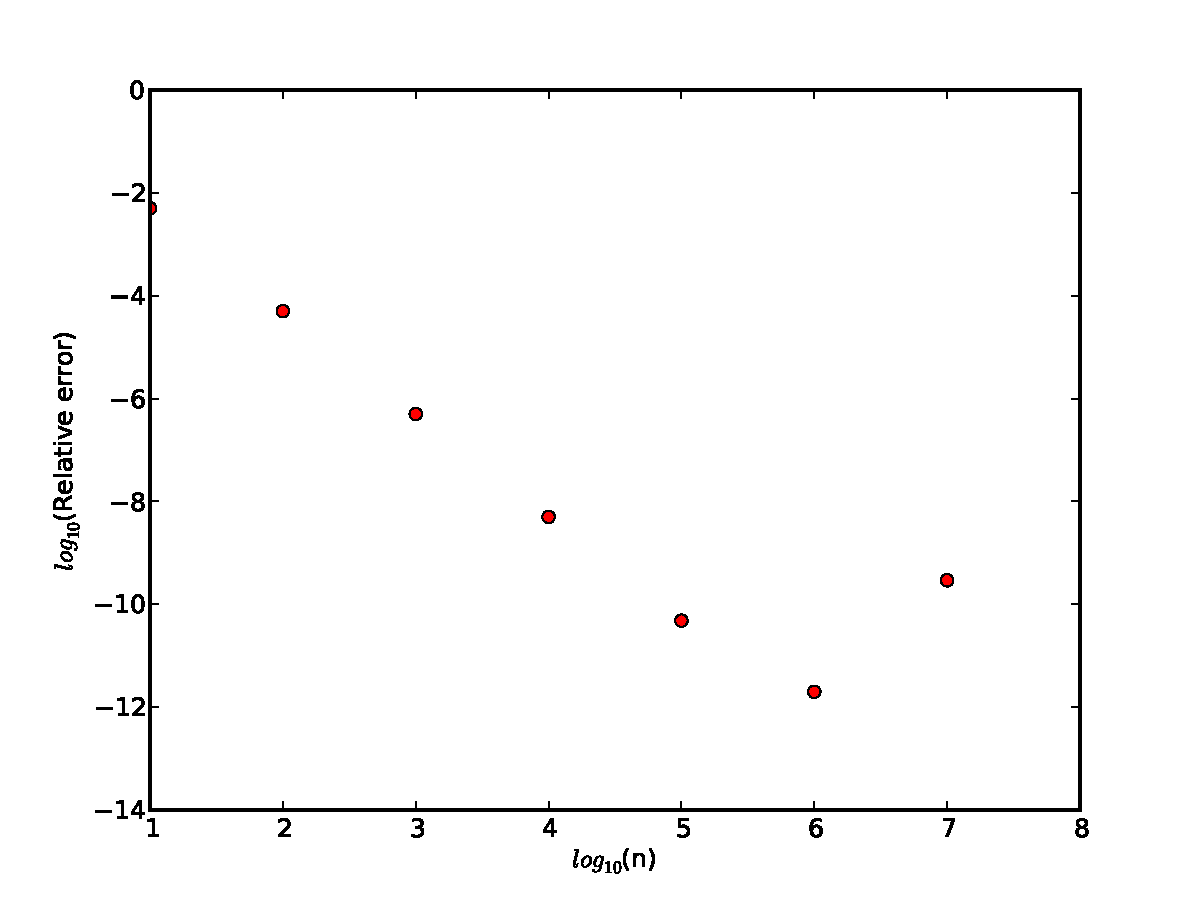
\includegraphics[scale=0.8]{Figures/error.pdf}
\caption{Log-log plot of the relative error as function of the number of integration points. Till approximately $n=10^6$, the relative error follows the predicted mathematical error of the trapezoidal rule. For higher numbers of integration points, numerical round off errors and loss of numerical precision give an increasing relative error.}\label{fig:error}
\end{figure}

The above example allows the student to also test the mathematical
error of the algorithm for the trapezoidal rule by changing the number
of integration points. The students get trained from day one to think
error analysis. Figure \ref{fig:error}  shows clearly the region where the
relative error starts increasing.  The mathematical error which
follows the trapezoidal rule goes as $O(h^2)$ where $h$ is the chosen
numerical step size. It is proportional to the inverse of the number of integration points $n$, that is $h\propto 1/n$.

Before numerical round-off errors and loss of
numerical precision kick in (near $h\sim 10^{-6}$) we see that the
relative error in the log-log plot has a slope which follows the
mathematical error.

There are several additional benefits here. The general learning outcomes on computing can be included as in for example the following ways. We
can easily bake in how to structure a code in terms of
functions and modules, or how to read input data flexibly from the
command line or how to write unit tests etc.  The conventions and
techniques outlined here will save students a lot of time when one
extends incrementally software over time, from simpler to more
complicated problems. In the next subsection we show how algorithms
for solving sets of ordinary differential equations and finding
eigenvalues can be reused in different courses with minor
modifications only.




\chapter{Teaching Mechanics with Computational Exercises and Projects}


We assume that our students know how to solve and study systems of
ordinary differential with initial conditions only. Later in this
section we will venture into two-point boundary value problems that
can be studied and solved with eigenvalue solvers.

Let us start with initial value problems and ordinary differential
equations. Such equations appear in a wealth of physics
applications. Typical examples students will encounter are the
classical pendulum in a mechanics course, an RLC circuit in the course on
electromagnetism, the modeling of the Solar system in an Astrophysics
course and many other cases.  The essential message is that, with
properly scaled equations, students can use essentially the
same algorithms to solve these problems, either starting with
a simple modified Euler algorithm or a Runge-Kutta class of
algorithms or the so-called Verlet class of algorithms, to mention a few.

The idea is that algorithms students develop and use in one course can be
reused in other courses.  This allows  students to make the
relevant abstractions discussed above, opening up for a much wider
range of applicabilities.

Here we look at two familiar cases from
mechanics and electromagnetism, the equations for the classical
pendulum and those for an RLC circuit.  When properly scaled, these
equations are essentially the same. To scale equations,
either in terms of dimensionless variables or appropriate variables,
is an important aspect which allows the students to see the potential
for abstractions and hopefully see how the problems studied in say a
mechanics course can be transferred to other fields.

The classical pendulum with damping and external force as it could
appear in a mechanics course is given by the following equation of
motion for the angle $\theta$ as function of time $t$
\[
  ml\frac{d^2\theta}{dt^2}+\nu\frac{d\theta}{dt}  +mgsin(\theta)=Acos(\omega t),
\]
where $m$ is its mass, $l$ the length, $\nu$ a damping factor and $A$
the amplitude of an applied external source with frequency
$\omega$. The solution of this type of equations (second-order
differential equations with given initial conditions) is something the
students encounter the first semester thorugh the courses IN1900 and
MAT-INF1100 at the University of Oslo. At Michigan State University
there is now a compulsory course for physics majors that includes many
of these elements.  With this background, students are already familiar with
the numerical solution and visualization of such equations.
If we now
move to a course on electromagnetism, we encounter almost the same
equation for an RLC circuit, namely
\[
L\frac{d^2Q}{dt^2}+\frac{Q}{C}+R\frac{dQ}{dt}=Acos(\omega t),
\]
where $L$ is the inductance, $R$ the applied resistance, $Q$ the
time-dependent charge and $C$ the capacitance.

Let us consider first the classical pendulum equations with damping and an
external force and define the scaled velocity $\hat{v}$ as
\[
   \frac{d\theta}{d\hat{t}} =\hat{v},
\]
where we have defined a dimensionless time variable $\hat{t}$. With
the equation for the velocity we can rewrite the second-order
differential in terms of two coupled first-order differential
equations where the second equation represents the acceleration
\[
   \frac{d\hat{v}}{d\hat{t}} =Acos(\hat{\omega} \hat{t})-\hat{v}\xi-\sin(\theta).
\]
We have scaled the  equations with $\omega_0=\sqrt{g/l}$,
$\hat{t}=\omega_0 t$ and $\xi = mg/\omega_0\nu$. The frequency
$\omega_0$ defines a so-called natural frequency defined by the
gravitational acceleration $g$ and the length of the pendulum $l$. The
frequency $\hat{\omega}= \omega/\omega_0$.  In a similar way, our RLC
circuit can now be rewritten in terms of two coupled first-order
differential equations,
\[
   \frac{dQ}{d\hat{t}} =\hat{I},
\]
and
\[
   \frac{d\hat{I}}{d\hat{t}} =Acos(\hat{\omega} \hat{t})-\hat{I}\xi-Q,
\]
with $\omega_0=1/\sqrt{LC}$, $\hat{t}=\omega_0 t$ and $\xi =
CR\omega_0$. Here we see that the natural frequency is defined in
terms of the physical parameters $L$ and $C$.

The equations are essentially the same, the main differences reside in
the different scaling constants and the introduction of a non-linear
term for the angle $\theta$ in the pendulum equation. The differential
solver the students end up writing in the mechanics course (which
comes normally before the course on electromagnetism) can then be
reused in the electromagnetism course, with a great potential for
further abstraction.

Let us now move to another frequently encountered problem in several
physics courses, namely that of a two-point boundary value problem. In
the examples below we will see again that if the equations are
properly scaled, we can reuse the same algorithm for solving different
physics problems. Here we will start with the equations for a buckling
beam (a case which can be found in a mechanics course or a course on
mathematical methods in physics). Thereafter, with a simple change of
variables and constants, the same problem can be used to study a
quantum mechanical particle confined to move in an infinite potential
well.  By simply changing the diagonal matrix elements of the
discretized differential equation problem, we can study particles that
move in a harmonic oscillator potential or other types of
quantum-mechanical one-body or selected two-body problems.  With
slight modifications to the matrix that results from the
discretization of a second derivative, we can study Poisson's equation
in one dimension, a problem of relevance in
electromagnetism.

Let us start with the buckling beam. This is a two-point boundary
value problem
\[
R \frac{d^2 u(x)}{dx^2} = -F u(x),
\]
where $u(x)$ is the vertical displacement, $R$ is a material specific
constant, $F$ is the applied force and $x \in [0,L]$ with $u(0)=u(L)=0$.
We scale the equation with $x = \rho L$ and $\rho \in [0,1]$ and get
(note that we change from $u(x)$ to $v(\rho)$)
\[
\frac{d^2 v(\rho)}{dx^2} +K v(\rho)=0,
\]
which is, when discretized (see below), nothing but a standard eigenvalue problem with $K=
FL^2/R$. Here we can assume that either the force $F$ or the material
specific rigidity $R$ are unknown.  If we replace $R=-\hbar^2/2m$ and
$-F=\lambda$, we have the quantum mechanical variant for a particle
moving in a well with infinite walls at the endpoints.  The way to
solve these equations numerically is to discretize the second
derivative and the right hand side as
\[
    -\frac{v_{i+1} -2v_i +v_{i-i}}{h^2}=\lambda v_i,
\]
with $i=1,2,\dots, n$. Here $h$ is the step size which is defined by
the number of integration (or mesh) points.  We need to add to this
system the two boundary conditions $v(0) =v_0$ and $v(1) = v_{n+1}$,
although they are not needed in the solution of the equations since
their values are known.  For all integration points $i=1,2,\dots, n$
the set of equations to solve result in a so-called tridiagonal
Toeplitz matrix ( a special case from the discretized second
derivative)
\[
    \mathbf{A} = \frac{1}{h^2}\begin{bmatrix}
                          2 & -1 &  &   &  & \\
                          -1 & 2 & -1 & & & \\
                           & -1 & 2 & -1 & &  \\
                           & \dots   & \dots &\dots   &\dots & \dots \\
                           &   &  &-1  &2& -1 \\
                           &    &  &   &-1 & 2 \\
                      \end{bmatrix}
\]
and with the corresponding vectors $\mathbf{v} = (v_1, v_2,
\dots,v_n)^T$ allows us to rewrite the differential equation as a
standard eigenvalue problem
\[
   \mathbf{A}\mathbf{v} = \lambda\mathbf{v}.
\]
The tridiagonal Toeplitz matrix has analytical eigenpairs,
providing us thereby with an invaluable check on the equations to be
solved.


\chapter{From Mechanics to Electromagnetism}

A simple rewrite allows for the reuse in linear algebra problems for
solution of say Poisson's equation in electromagnetism, or the
diffusion equation in one dimension. To see this and how the same matrix can be used in a course in electromagnetism, let us consider
Poisson's equation.
We assume that
the electrostatic potential $\Phi$ is generated by a localized charge
distribution $\rho (\mathbf{r})$.   In three dimensions
the pertinent equation reads
\[
\nabla^2 \Phi = -4\pi \rho (\mathbf{r}).
\]
With a spherically symmetric potential $\Phi$ and charge distribution $\rho (\mathbf{r})$ and using spherical coordinates,  the relevant
equation to solve
simplifies to a one-dimensional equation in $r$, namely
\[
\frac{1}{r^2}\frac{d}{dr}\left(r^2\frac{d\Phi}{dr}\right) = -4\pi \rho(r),
\]
which can be rewritten via a substitution $\Phi(r)= \phi(r)/r$ as
\[
\frac{d^2\phi}{dr^2}= -4\pi r\rho(r).
\]
The inhomogeneous term $f$ or source term is given by the charge distribution
$\rho$  multiplied by $r$ and the constant $-4\pi$.

We can  rewrite this equation by letting $\phi\rightarrow u$ and
$r\rightarrow x$.  Scaling again the equations and replacing the right hand side with a function $f(x)$, we can rewrite the
equation as
\[
-u''(x) = f(x).
\]
Our scaling gives us again $x\in [0,1]$ and the two-point boundary value problem
with $u(0)=u(1)=0$. With $n+1$ integration points and
the step length defined as $h=1/(n)$ and replacing the continuous function $u$ with its discretized version $v$, we get
the following equation
\begin{equation*}
   -\frac{v_{i+1}+v_{i-1}-2v_i}{h^2} = f_i  \hspace{0.5cm} \mathrm{for} \hspace{0.1cm} i=1,\dots, n,
\end{equation*}
where $f_i=f(x_i)$.
Bringing up again the tridiagonal Toeplitz matrix,
\[
    \mathbf{A} = \frac{1}{h^2}\begin{bmatrix}
                           2& -1& 0 &\dots   & \dots &0 \\
                           -1 & 2 & -1 &0 &\dots &\dots \\
                           0&-1 &2 & -1 & 0 & \dots \\
                           & \dots   & \dots &\dots   &\dots & \dots \\
                           0&\dots   &  &-1 &2& -1 \\
                           0&\dots    &  & 0  &-1 & 2 \\
                      \end{bmatrix},
\]
our problem becomes now a classical linear algebra problem
\[
\mathbf{A}\mathbf{v}=\mathbf{f},
\]
with the unknown function $\mathbf{v}$. Using standard LU
decomposition algorithms \cite{GolubVanLoan} (here one can use
the so-called Thomas algorithm which reduces the number of floating
point operations to $O(n)$) one can easily find the solution to this
problem.

These examples demonstrate how one can, with a discretized second
derivative, solve physics problems that arise in different
undergraduate courses using standard linear algebra and eigenvalue
algorithms and ordinary differential equations, allowing thereby
teachers to focus on the interesting physics. Many of these problems
can easily be linked up with ongoing research. This opens up for many
interesting perspectives in physics education. We can bring in at a
much earlier stage in our education basic research elements and
perhaps even link with ongoing research during the first year of
undergraduate studies.

Instead of focusing on tricks and mathematical manipulations to solve
the continuous problems for those few case where an analytical
solution can be found, the discretization of the continuous problem
opens up for studies of many more interesting and realistic problems.
However, we have seen that in order to verify and validate our codes,
the existence of analytical solutions offer us an invaluable test of
our algorithms and programs. The analytical results can either be
included explicitely or via symbolic software like Python's Sympy package.
Thus, computing stands indeed for solving scientific problems using
all possible tools, including symbolic computing, computers and
numerical algorithms, numerical experiments (as well as real
experiments if possible) and analytical paper and pencil solutions.


\chapter{And then into Quantum Physics and Quantum Mechanics}


Let us start with the buckling beam. This is a two-point boundary
value problem
\[
R \frac{d^2 u(x)}{dx^2} = -F u(x),
\]
where $u(x)$ is the vertical displacement, $R$ is a material specific
constant, $F$ is the applied force and $x \in [0,L]$ with $u(0)=u(L)=0$.
We scale the equation with $x = \rho L$ and $\rho \in [0,1]$ and get
(note that we change from $u(x)$ to $v(\rho)$)
\[
\frac{d^2 v(\rho)}{dx^2} +K v(\rho)=0,
\]
which is, when discretized (see below), nothing but a standard eigenvalue problem with $K=
FL^2/R$. Here we can assume that either the force $F$ or the material
specific rigidity $R$ are unknown.  If we replace $R=-\hbar^2/2m$ and
$-F=\lambda$, we have the quantum mechanical variant for a particle
moving in a well with infinite walls at the endpoints.  The way to
solve these equations numerically is to discretize the second
derivative and the right hand side as
\[
    -\frac{v_{i+1} -2v_i +v_{i-i}}{h^2}=\lambda v_i,
\]
with $i=1,2,\dots, n$. Here $h$ is the step size which is defined by
the number of integration (or mesh) points.  We need to add to this
system the two boundary conditions $v(0) =v_0$ and $v(1) = v_{n+1}$,
although they are not needed in the solution of the equations since
their values are known.  For all integration points $i=1,2,\dots, n$
the set of equations to solve result in a so-called tridiagonal
Toeplitz matrix ( a special case from the discretized second
derivative)
\[
    \mathbf{A} = \frac{1}{h^2}\begin{bmatrix}
                          2 & -1 &  &   &  & \\
                          -1 & 2 & -1 & & & \\
                           & -1 & 2 & -1 & &  \\
                           & \dots   & \dots &\dots   &\dots & \dots \\
                           &   &  &-1  &2& -1 \\
                           &    &  &   &-1 & 2 \\
                      \end{bmatrix}
\]
and with the corresponding vectors $\mathbf{v} = (v_1, v_2,
\dots,v_n)^T$ allows us to rewrite the differential equation as a
standard eigenvalue problem
\[
   \mathbf{A}\mathbf{v} = \lambda\mathbf{v}.
\]
The tridiagonal Toeplitz matrix has analytical eigenpairs,
providing us thereby with an invaluable check on the equations to be
solved.

If we stay with quantum mechanical one-body problems (or
special interacting two-body problems) adding a potential along the
diagonal elements allows us to reuse this problem for many types of physics
cases.  To see this, let us assume we are interested in the solution
of the radial part of Schr\"odinger's equation for one electron. This
equation reads
\[
  -\frac{\hbar^2}{2 m} \left ( \frac{1}{r^2} \frac{d}{dr} r^2
  \frac{d}{dr} - \frac{l (l + 1)}{r^2} \right )R(r)
     + V(r) R(r) = E R(r).
\]
Suppose in our case $V(r)$ is the harmonic oscillator potential
$(1/2)kr^2$ with $k=m\omega^2$ and $E$ is the energy of the harmonic
oscillator in three dimensions.  The oscillator frequency is $\omega$
and the energies are
\[
E_{nl}=  \hbar \omega \left(2n+l+\frac{3}{2}\right),
\]
with $n=0,1,2,\dots$ and $l=0,1,2,\dots$.

Since we have made a transformation to spherical coordinates it means
that $r\in [0,\infty)$. The quantum number $l$ is the orbital momentum
  of the electron.  In order to find analytical solutions for this
  problem, we would substitute $R(r) = (1/r) u(r)$ (which gives
  $u(0)=u(\infty)=0$ and thereby easier boundary conditions) and
  obtain
\[
  -\frac{\hbar^2}{2 m} \frac{d^2}{dr^2} u(r)
       + \left ( V(r) + \frac{l (l + 1)}{r^2}\frac{\hbar^2}{2 m}
                                    \right ) u(r)  = E u(r) .
\]
The boundary conditions are $u(0)=0$ and $u(\infty)=0$.

In order to scale the equations, we introduce a dimensionless variable $\rho = (1/\alpha) r$
where $\alpha$ is a constant with dimension length and get
\[
  -\frac{\hbar^2}{2 m \alpha^2} \frac{d^2}{d\rho^2} v(\rho)
       + \left ( V(\rho) + \frac{l (l + 1)}{\rho^2}
         \frac{\hbar^2}{2 m\alpha^2} \right ) v(\rho)  = E v(\rho) .
\]
Let us choose $l=0$ for the mere sake of simplicity.
Inserting $V(\rho) = (1/2) k \alpha^2\rho^2$ we end up with
\[
  -\frac{\hbar^2}{2 m \alpha^2} \frac{d^2}{d\rho^2} v(\rho)
       + \frac{k}{2} \alpha^2\rho^2v(\rho)  = E v(\rho).
\]
We multiply thereafter with $2m\alpha^2/\hbar^2$ on both sides and obtain
\[
  -\frac{d^2}{d\rho^2} v(\rho)
       + \frac{mk}{\hbar^2} \alpha^4\rho^2v(\rho)  = \frac{2m\alpha^2}{\hbar^2}E v(\rho) .
\]

A natural length scale comes out automatically when scaling. To see this, since $\alpha$ is constant we are left to determine, 
we determine $\alpha$ by requiring that
\[
\frac{mk}{\hbar^2} \alpha^4 = 1.
\]
This defines a natural length scale in terms of the various physical
constants that determine the equation.  The final expression, inserting $k=m\omega^2$ is
\[
\alpha = \left(\frac{\hbar}{m\omega}\right)^{1/2}.
\]
If we were to replace the harmonic oscillator potential with the
attractive Coulomb interaction from the hydrogen atom, the  parameter $\alpha$ would equal the Bohr
radius $a_0$.  This way students see the general properties of a
two-point boundary value problem and can reuse the code they developed
for a mechanics course to the subsequent quantum mechanical course.

Defining
\[
\lambda = \frac{2m\alpha^2}{\hbar^2}E,
\]
we can rewrite Schroedinger's equation as
\[
  -\frac{d^2}{d\rho^2} v(\rho) + \rho^2v(\rho)  = \lambda v(\rho) .
\]
This is similar to the equation for a buckling beam, except for the
potential term.  In three dimensions with our scaling, the eigenvalues for $l=0$ are
$\lambda_0=3,\lambda_1=7,\lambda_2=11,\dots .$

If we  define first the diagonal matrix element
\[
   d_i=\frac{2}{h^2}+V_i,
\]
and the non-diagonal matrix element
\[
   e_i=-\frac{1}{h^2},
\]
we can rewrite the Schr\"oedinger equation as
\[
d_iu_i+e_{i-1}v_{i-1}+e_{i+1}v_{i+1}  = \lambda v_i,
\]
where $v_i$ is unknown and $i=1,2,\dots, n$. We can reformulate the
latter equation as a matrix eigenvalue problem
\[
    \begin{bmatrix} d_1 & e_1 & 0   & 0    & \dots  &0     & 0 \\
                                e_1 & d_2 & e_2 & 0    & \dots  &0     &0 \\
                                0   & e_2 & d_3 & e_3  &0       &\dots & 0\\
                                \dots  & \dots & \dots & \dots  &\dots      &\dots & \dots\\
                                0   & \dots & \dots & \dots  &\dots       &d_{n-1} & e_{n-1}\\
                                0   & \dots & \dots & \dots  &\dots       &e_{n-1} & d_{n}
             \end{bmatrix}      \begin{bmatrix} v_{1} \\
                                                              v_{2} \\
                                                              \dots\\ \dots\\ \dots\\
                                                              v_{n}
             \end{bmatrix}=\lambda \begin{bmatrix}{c} v_{1} \\
                                                              v_{2} \\
                                                              \dots\\ \dots\\ \dots\\
                                                              v_{n}
             \end{bmatrix}
\]
or if we wish to be more detailed, we can write the tridiagonal matrix as
\[
    \begin{bmatrix} \frac{2}{h^2}+V_1 & -\frac{1}{h^2} & 0   & 0    & \dots  &0     & 0 \\
                                -\frac{1}{h^2} & \frac{2}{h^2}+V_2 & -\frac{1}{h^2} & 0    & \dots  &0     &0 \\
                                0   & -\frac{1}{h^2} & \frac{2}{h^2}+V_3 & -\frac{1}{h^2}  &0       &\dots & 0\\
                                \dots  & \dots & \dots & \dots  &\dots      &\dots & \dots\\
                                0   & \dots & \dots & \dots  &\dots       &\frac{2}{h^2}+V_{n-1} & -\frac{1}{h^2}\\
                                0   & \dots & \dots & \dots  &\dots       &-\frac{1}{h^2} & \frac{2}{h^2}+V_{n}
             \end{bmatrix}.
\]

The following Python code sets up the matrix to diagonalize by defining
the minimun and maximum values of $r$ with a maximum value of
integration points. It plots the eigenfunctions of the three lowest
eigenstates.
\begin{lstlisting}
#Program which solves the one-particle Schrodinger equation
#for a potential specified in function
#potential().

from  matplotlib import pyplot as plt
import numpy as np
#Function for initialization of parameters
def initialize():
    RMin = 0.0
    RMax = 10.0
    lOrbital = 0
    Dim = 400
    return RMin, RMax, lOrbital, Dim
# Harmonic oscillator potential
def potential(r):
    return 0.5*r*r

#Get the boundary, orbital momentum and number of integration points
RMin, RMax, lOrbital, Dim = initialize()

#Initialize constants
Step    = RMax/(Dim)
DiagConst = 2.0/ (Step*Step)
NondiagConst =  -1.0 / (Step*Step)
OrbitalFactor = lOrbital * (lOrbital + 1.0)

#Calculate array of potential values
v = np.zeros(Dim)
r = np.linspace(RMin,RMax,Dim)
for i in range(Dim):
    r[i] = RMin + (i+1) * Step;
    v[i] = potential(r[i]) + OrbitalFactor/(r[i]*r[i]);

#Setting up a tridiagonal matrix and finding eigenvectors and eigenvalues
Matrix = np.zeros((Dim,Dim))
Matrix[0,0] = DiagConst + v[0];
Matrix[0,1] = NondiagConst;
for i in xrange(1,Dim-1):
    Matrix[i,i-1]  = NondiagConst;
    Matrix[i,i]    = DiagConst + v[i];
    Matrix[i,i+1]  = NondiagConst;
Matrix[Dim-1,Dim-2] = NondiagConst;
Matrix[Dim-1,Dim-1] = DiagConst + v[Dim-1];
# diagonalize and obtain eigenvalues, not necessarily sorted
EigValues, EigVectors = np.linalg.eig(Matrix)
# sort eigenvectors and eigenvalues
permute = EigValues.argsort()
EigValues = EigValues[permute]
EigVectors = EigVectors[:,permute]
# now plot the results for the three lowest lying eigenstates
for i in range(3):
    print(EigValues[i])
FirstEigvector = EigVectors[:,0]
SecondEigvector = EigVectors[:,1]
ThirdEigvector = EigVectors[:,2]
plt.plot(r, FirstEigvector**2 ,'b-',r, SecondEigvector**2 ,'g-',r, ThirdEigvector**2 ,'r-')
plt.axis([0,4.6,0.0, 0.025])
plt.xlabel(r'$r$')
plt.ylabel(r'Radial probability $r^2|R(r)|^2$')
plt.title(r'Radial probability distributions for three lowest-lying states')
plt.savefig('eigenvector.pdf')
plt.show()
\end{lstlisting}


The last example shows the potential of combining numerical algorithms with analytical results (or eventually symbolic calculations), allowing thereby students to test their physics understanding. One can easily switch to other potentials by simply redefining the potential function. For example, a finite box potential can easily be defined as
\begin{lstlisting}
# Finite depth and range box potential, with strength V and range a
def potential(r):
    if r >= 0.0 and r <= 10.0:
        V = -0.05
    else:
        V =0.0
    return V
\end{lstlisting}
Thereafter, the students can explore the role of the potential depth
and the range of the potential. Analyzing the eigenvectors gives
additional information about the spatial degrees of freedom in terms
of different potentials.  The possibility to visualize the results immediately, as shown in figure \ref{fig:eigenvector}, aids in providing students with a deeper understanding of the relevant physics.

This example contains also many of the
computing learning outcomes we discussed above, in addition to those
related to the physics of a particular system. We see that, by proper
scaling, the students can make further abstractions and explore other
physics cases easily where no analytical solutions are known. With
unit testing and analytical results they can validate and verify their
algorithms.
\begin{figure}
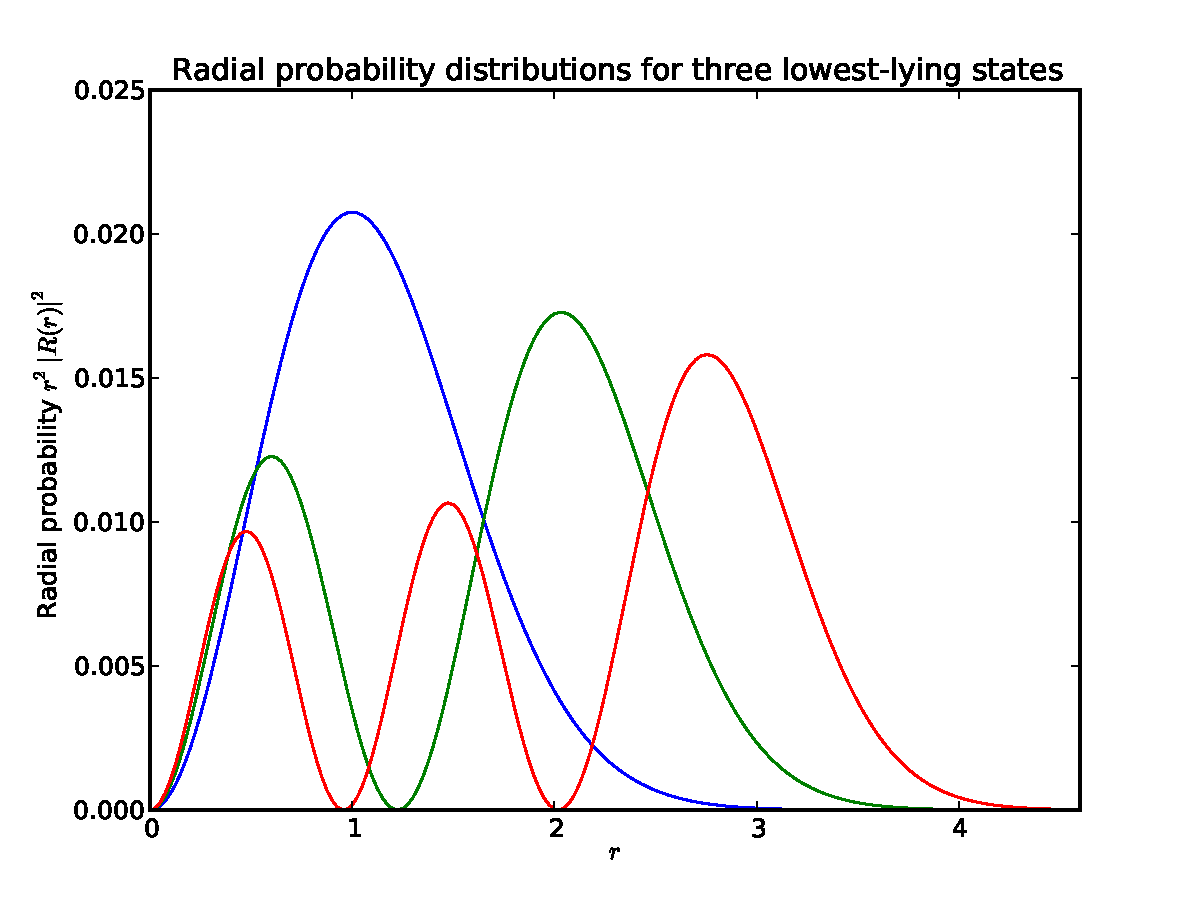
\includegraphics[scale=0.8]{Figures/eigenvector.pdf}
\caption{Plot of the eigenfunctions of the three lowest-lying eigenvalues for a harmonic oscillator problem in three dimensions. The students can easily change the type of potential and explore the physics that arises from these potentials.}\label{fig:eigenvector}
\end{figure}



The above example allows the student to test the mathematical error of
the algorithm for the eigenvalue solver by simply changing the number
of integration points. Again, as discussed above in connection with
the trapezoidal rule, the students get trained to develop an
understanding of the error analysis and where things can go wrong. The
algorithm can be tailored to any kind of one-particle problem used in
quantum mechanics.


\chapter{Statistical and Thermal Physics}




\end{document}





